\documentclass{article}
% Language setting
% Replace `russian' with e.g. `spanish' to change the document language
\usepackage[russian]{babel}

% Set page size and margins
% Replace `letterpaper' with `a4paper' for UK/EU standard size
\usepackage[letterpaper,top=2cm,bottom=2cm,left=3cm,right=3cm,marginparwidth=1.75cm]{geometry}

% Useful packages
\usepackage{amsmath}
\usepackage{graphicx}
\usepackage[colorlinks=true, allcolors=blue]{hyperref}

\title{Вариант 6}
\author{Тема:Хеш-Таблицы}

\begin{document}
\maketitle

\section{Ход работы: }
\subsection{Код Программы:}

\begin{verbatim}
#include <iostream>
#include <list>

using namespace std;

class HashTable{
private:
	list<int> *table;
	int total_elements;

	// Хэш-функция для вычисления хэша для значения:
	int getHash(int key){
		return key % total_elements;
	}

public:
	// Конструктор для создания хэш-таблицы с 'n' индексами:
	HashTable(int n){
		total_elements = n;
		table = new list<int>[total_elements];
	}

	// Вставка данных в хэш-таблицу:
	void insertElement(int key){
		table[getHash(key)].push_back(key);
	}

	// Удаление данных из хэш-таблицы:
	void removeElement(int key){
		int x = getHash(key);

		list<int>::iterator i;
		for (i = table[x].begin(); i != table[x].end(); i++) {
			//Проверьте, указывает ли итератор на требуемый элемент:
			if (*i == key)
				break;
		}

		// Если элемент был найден в списке, то удалите его:
		if (i != table[x].end())
			table[x].erase(i);
	}

	void printAll(){
		// Пройдите по каждому индексу:
		for (int i = 0; i < total_elements; i++){
			cout << "Index " << i << ": ";
			// Пройдите по списку по текущему индексу:
			for (int j : table[i])
				cout << j << " => ";

			cout << endl;
		}
	}
};

int main() {
	HashTable ht(3);
	int arr[10];
	for (int i = 0; i < 10; i++){
		cout << "[" << i + 1 << "]" << ": ";
		cin >> arr[i];
	}
	// Вставьте все данные в хэш-таблицу:
	for (int i = 0; i < 10; i++)
		ht.insertElement(arr[i]);

	cout << "..:: Hash Table ::.." << endl;
	ht.printAll();
	system("pause");
	return 0;
}
\end{verbatim}
\subsection{Код в работающем состоянии}
\begin{figure}[h]
	\centering
	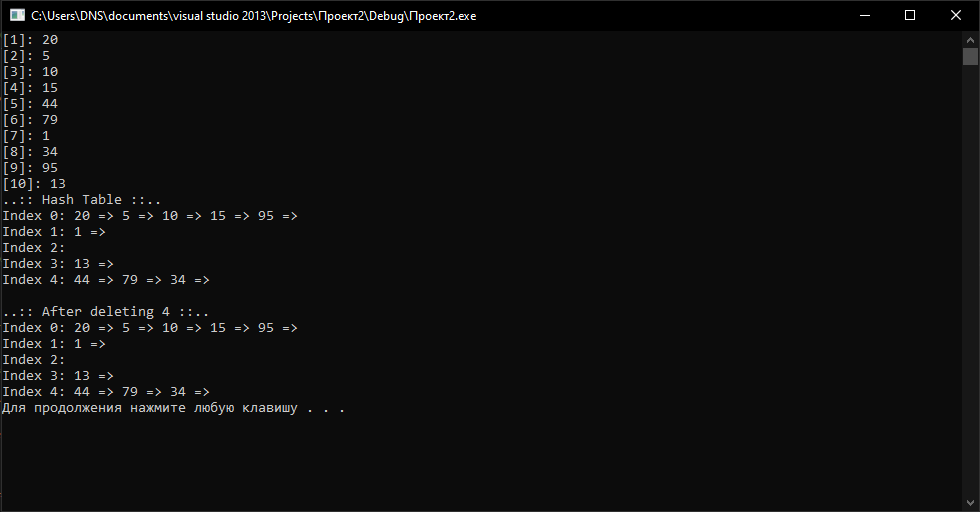
\includegraphics[width=0.4\textwidth]{index5.png}
	\caption{Хеш-Таблица с 5 индексами}\label{fig:par}
\end{figure}
\begin{figure}[h]
	\centering
	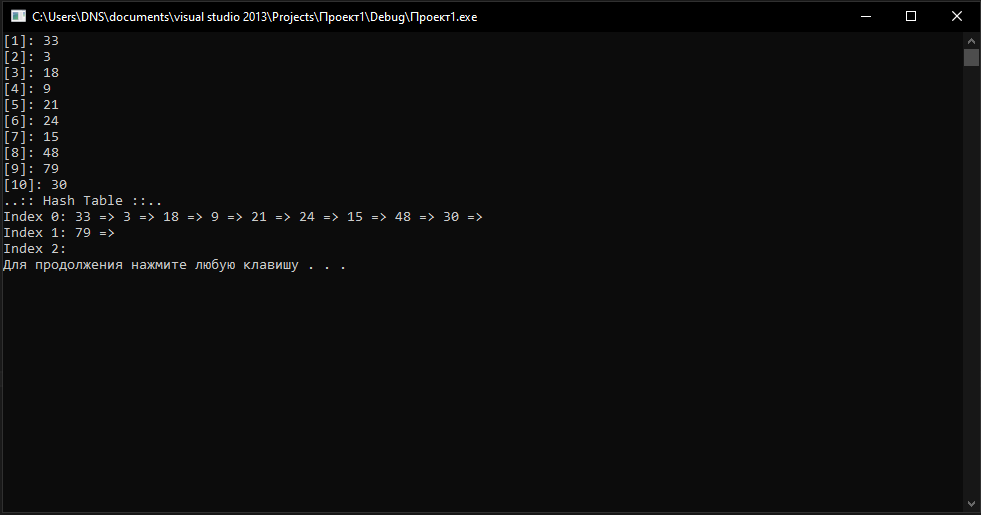
\includegraphics[width=0.4\textwidth]{Index3.png}
	\caption{Хеш-Таблица с 3 индексами}\label{fig:par}
\end{figure}


\bibliographystyle{alpha}

\bibliography{sample}
Информации о Хеш-Таблицах:https://habr.com/ru/post/509220/
\end{document}